\section{Isolation Comparison Study}
\label{sec:IsolationStudy}

In order to check that the definition of isolation (Sections.~\ref{sec:electron_cuts},~\ref{sec:muon_cuts})
as well as the subsequent pileup corrections is robust we compare the $M_jj$ 
shapes between Data and Monte Carlo. The results are shown in Fig.~\ref{fig:IsoComp}.
The discrepancies are covered by the trigger efficiency corrections and the
associated 2\% systematic (Section.~\ref{sec:LeptonSelectionAndTriggerEfficiency})

%%%%%%%
\begin{figure}[h!] {\centering
\unitlength=0.33\linewidth
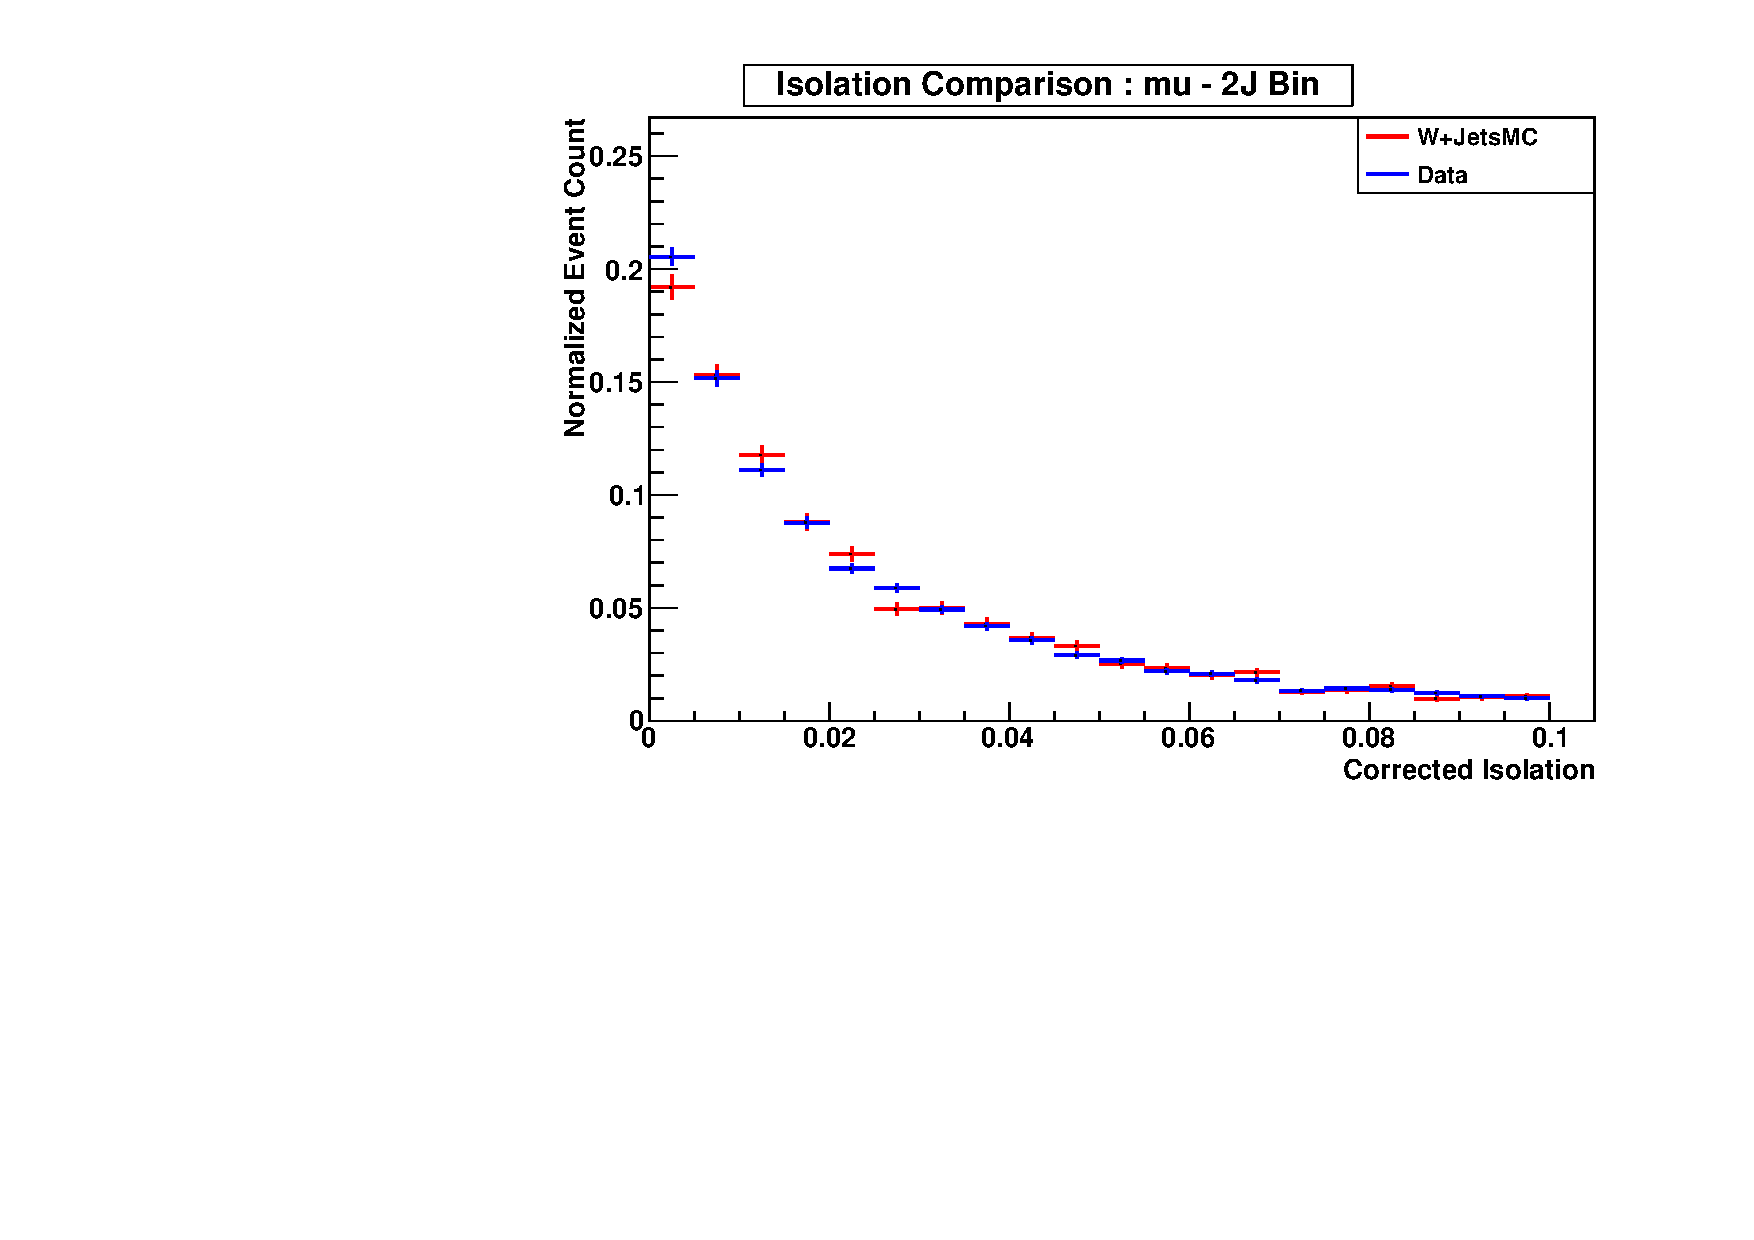
\includegraphics[width=0.48\textwidth]{figs/AdditionalStudies/IsoComp_mu2J.pdf}
\put(-0.80,0.0){(a)} 
\unitlength=0.33\linewidth
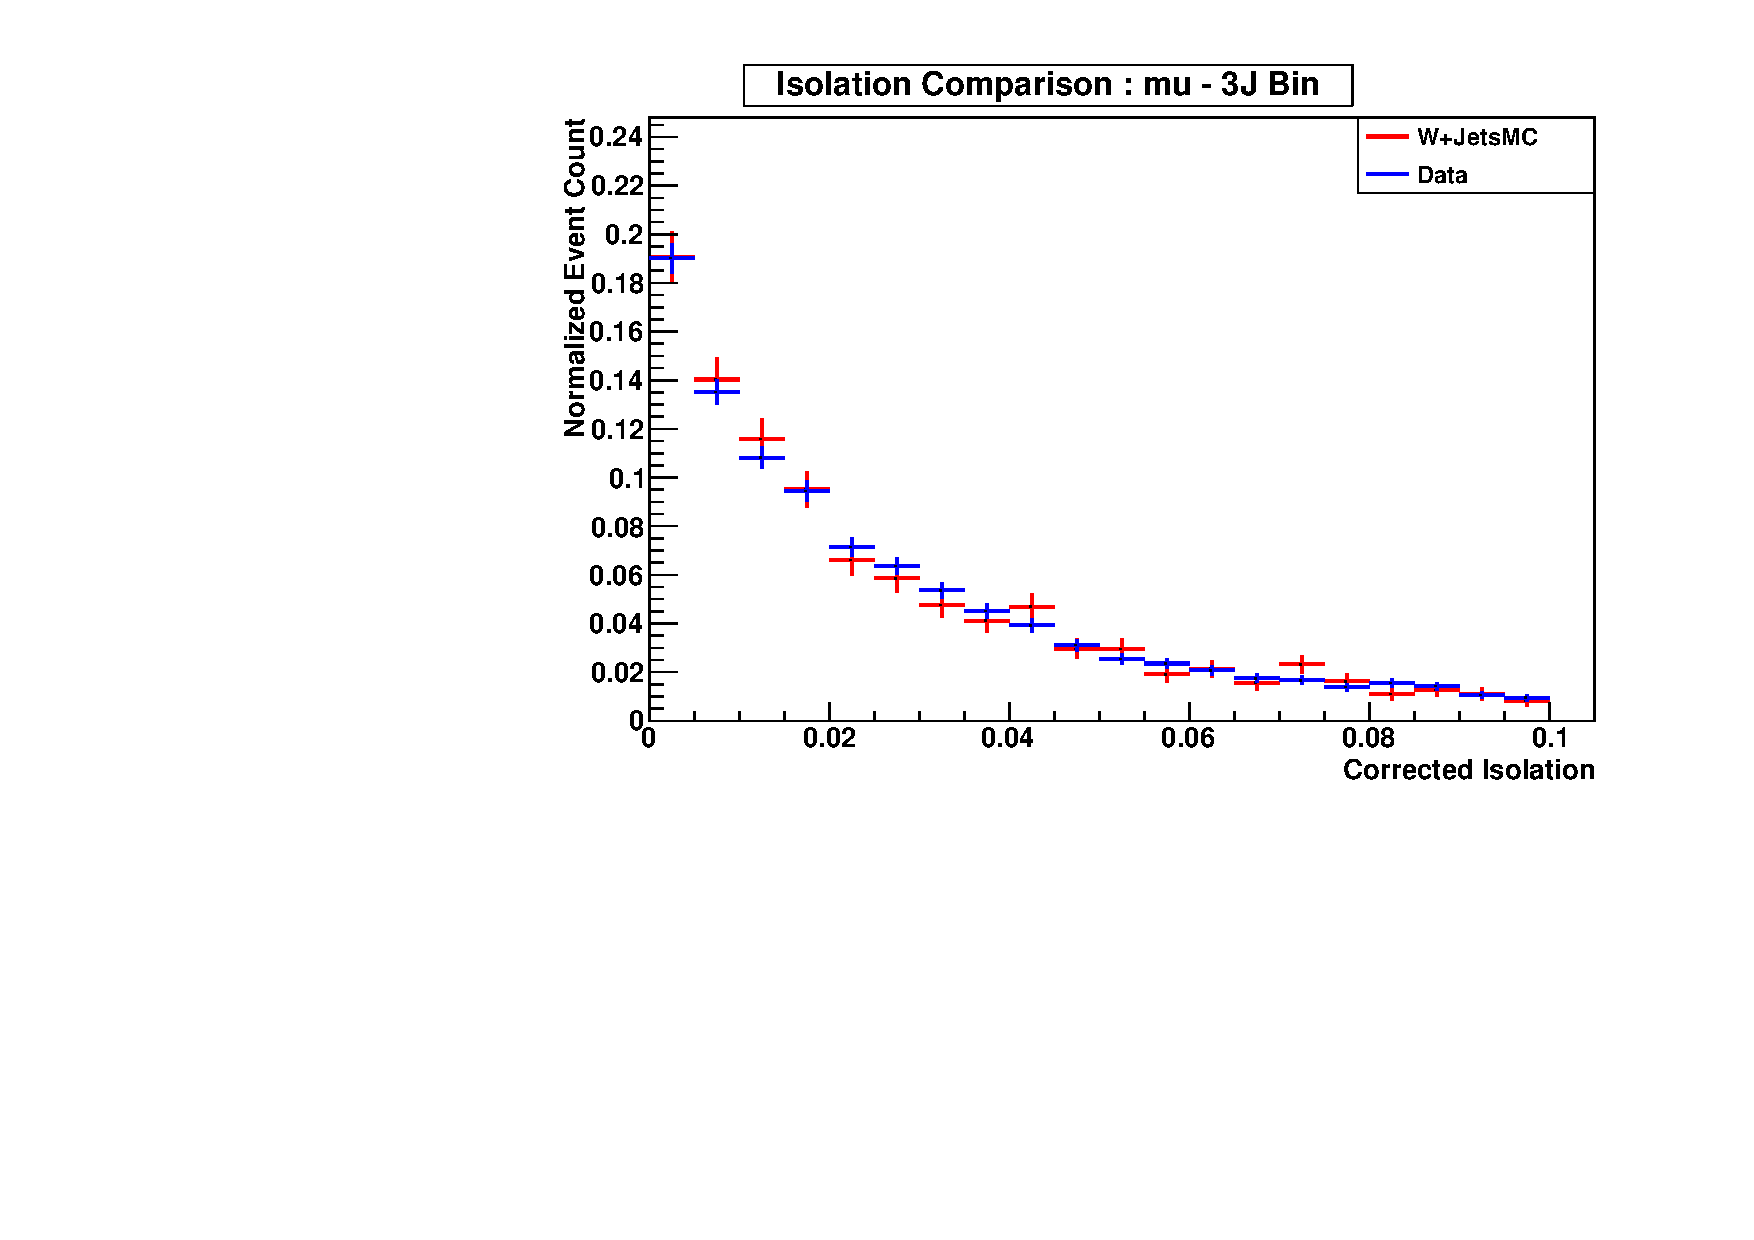
\includegraphics[width=0.48\textwidth]{figs/AdditionalStudies/IsoComp_mu3J.pdf}
\put(-0.80,0.0){(b)} \\
\unitlength=0.33\linewidth
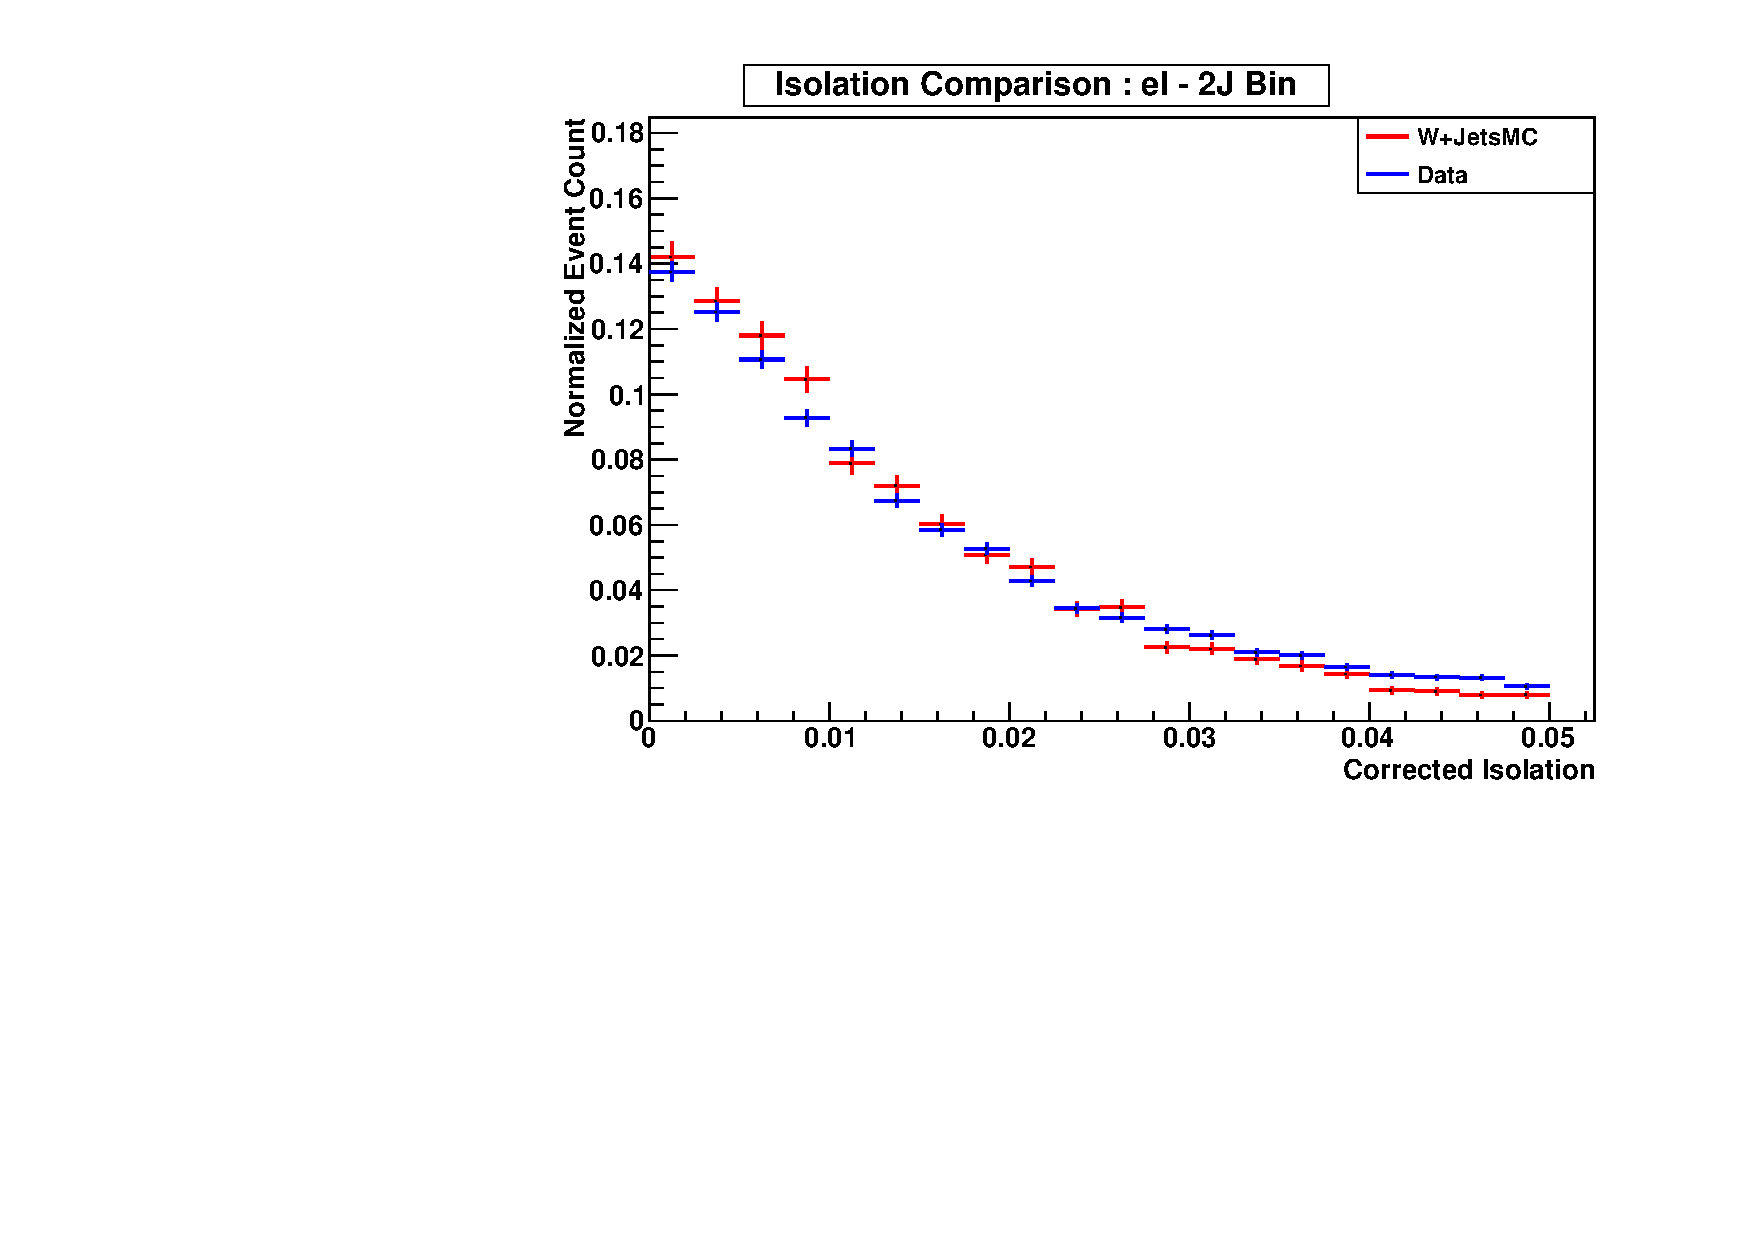
\includegraphics[width=0.48\textwidth]{figs/AdditionalStudies/IsoComp_el2J.pdf}
\put(-0.80,0.0){(c)} 
\unitlength=0.33\linewidth
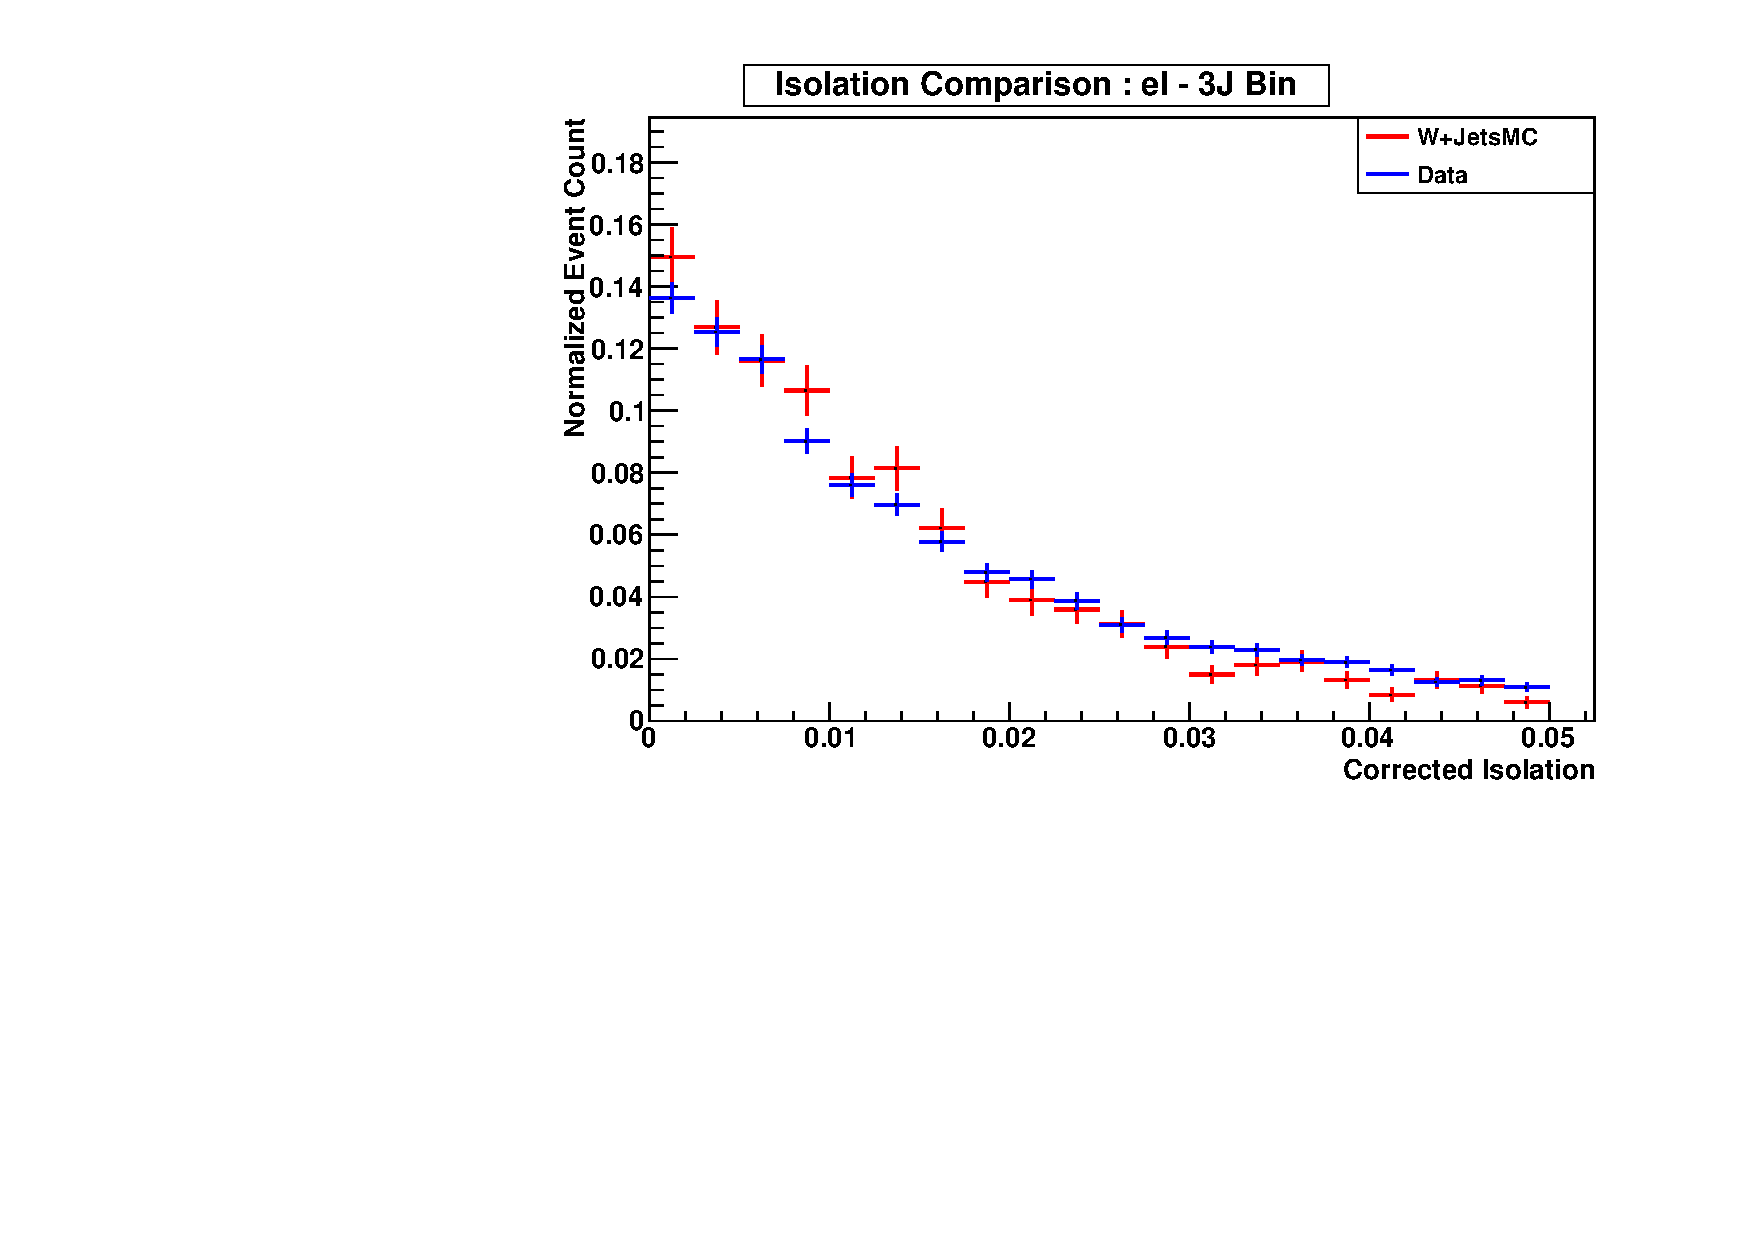
\includegraphics[width=0.48\textwidth]{figs/AdditionalStudies/IsoComp_el3J.pdf}
\put(-0.80,0.0){(d)} 
\caption{Comparison between Data and MC Isolation for: (a) muons - 2-jet bin, (b) muons - 3-jet bin, (c) electrons - 2-jet bin, (d) electrons - 3-jet bin.} 
\label{fig:IsoComp}
}
\end{figure}
%%%%%%%
